
\chapter{Обзор работы}
\label{chapter1}

В этой главе представлен общий обзор работы: уточнены цели и объяснены термины и понятия, присутствующие в решении
задачи. Также произведен обзор имеющихся результатов и сформулирована постановка задачи.

\section{Недоминирующая сортировка}

В данном разделе представлено определение недоминирующей сортировки и необходимые для ее понимания понятия.
Также рассмотрены случаи применения недоминирующей сортировки, которые обосновывают актуальность нового ускоренного
алгоритма недоминирующей сортировки.

\subsection{Определение}

Недоминирующая сортировка -- это процедура, которая ранжирует множество точек в многомерном пространсве $R^n$.
Если описывать неформально, то ее задача определить, какие точки \"лучше\" других. При этом допускается, что две точки 
могут быть одинаково \"хорошими\".

Для того, чтобы сформулировать определение недоминирующей сортировки, сначала надо определить, какие точки мы считаем 
\"лучше\" других. Для этого введем определение доминирования одной точки другой.

\textit{Определение.} В $M$-мерном пространстве, точка $A = (a_1,...,a_M)$ доминирует точку $B = (b_1,...,b_M)$
 тогда и только тогда, когда для всех $1 \leq i \leq M$ выполняется неравенство $a_i\leq b_i$, и существует такое $j$,
 что $a_j < b_j$.

\"Лучшими\" в данном контексте будут считаться точки, которые не доминируются ни одной другой точкой или, другми словами, 
лежащие на Парето-фронте. Однако часто бывают не только точки с парето-фронта, но и другие \"хорошие\" точки. Таким
образом мы приходим к определению процедуры недоминирующей сортировки.

\textit{Определение.} Недоминирующая сортировка множества точек $S$ в $M$-мерном пространстве — это процедура, которая 
назначает всем точкам из $S$ ранг. Все точки, которые не доминируются ни одной точкой из $S$ имеют ранг ноль. Точка 
имеет ранг $i+1$, если максимальный ранг среди доминирующих её точек равен $i$.

\subsection{Применение и актуальность}

Самый яркий пример применения процедуры недоминирующей сортировки -- алгоритмы многокритериальной оптимизации, особенно
эволюционные алгоритмы. Последние на каждой итерации генеририруют множество потенциальных решений и оценивают каждое 
решение по всем критериям. Если критериев $M$, то получается набор из $N$ $M$-мерных векторов, где $N$ -- число потенциальных 
решений. И эволюционому алгоритму на каждой итерации надо отобрать лучшие решения, для чего и требуется недоминирующая
сортировка.

Если каждый критерий для всех каждого потенциального решения считается достаточно долго, то время выполнения недоминирующей
сортировки становится неважным, так как асимптотика каждой итерации алгоритма зависит в основном от асимптотики времени 
подсчета критериев. Однако гораздо чаще встречаются задачи, в которых подсчет каждого критерия занимает время значительно 
меньшее, чем время, еобходимое для недоминирующей сортировки. Именно в таких случаях ускорение алгоритмов недоминирующей 
сортировки ускорит время выполнения итерации алгоритма, а следовательно и время выполнения всего алгоритма.

В настоящее время существует много алгоритмов недоминирующей сортировки. Но каждый из них имеет свои слабые стороны. Это 
означает, что существует возможность сделать алгоритм, который мог бы заранее предсказывать, время работы какого алгоритма 
на данном наборе точек будет меньше, и выбирать оптимальный. Более того есть возможность совместить идеи разных алгоритмов
в одном, который всегда будет работать не хуже существующих. Такие возможности делают проблему ускорения алгоритмов недоминирующей
сортировки еще более актуальной.

\section{Анализ существующих алгоритмов}

В данном разделе будут рассмотрена история развития алгоритмов недоминирующей сортировки. Особое внимание будет
уделено самым эффективным алгоритмам, которые применяются для гибридизации в данной работе. Они будут рассмотрены 
наиболее подробно.

\subsection{Наивные алгоритмы}

Опишем самый наивный алгоритм недоминирующей сортировки. Он перебирает все пары точек и сравненивает их по всем критериям.
После этого он присваивает нулевой ранг тем из них, которые не доминируются ни одной  другой точкой и отбрасывает их из 
множества. Данная процедура повторяется, пока в множестве остаются точки. Причем на каждом новом шаге присваивается 
новое значение ранга, на единицу больше, чем на предыдущем шаге. Рассмотрим время работы данного наивного алгоритма.
Пусть $N$ — это число точек, а $M$ — размерность пространства. Тогда сравнение всех пар точек по $M$ критериям займет 
$O(MN^2)$, а всего шагов алгоритма будет не больше, чем максимальное число рангов -- $N$. Таким образом, время работы
данного алгоритма не превышает $O(MN^3)$, причем эта оценка достигается в худшем случае при максимальном числе рангов
в сортируемом множестве.

В работе Кунга и др. \cite{Kung} предлагается алгоритм определения множества недоминируемых точек, при этом его
вычислительная сложность составляет $O(N log^{M-1} N)$. Этот алгоритм возможно использовать для выполнения недоминирующей 
сортировки аналагично вышеописанному алгоритму. Сначала в множестве $S$ алгоритм Кунга находит множество точек с рангом $0$. 
Затем алгоритм Кунга запускается на оставшемся множестве точек, и получившемуся множеству точек присваивается ранг $1$. 
Процесс выполняется до тех пор, пока имеются точки, которым не присвоен ранг. Описанная процедура в худшем случае 
выполняется за $O(N^2 log^{M-1} N)$, если максимальный ранг точки равен $O(N)$.

Также существует много других алгоритмов, асиптотика которых равна $O(MN^2)$, например, алгоритм ENS Жанга и др.~\cite{Zhang}.

\subsection{Алгоритмы <<Разделяй и властвуй>>}

Йенсен \cite{Jensen} впервые предложил алгоритм недоминирующей сортировки с вычислительной сложностью
$O(N log^{M-1} N)$. Однако, как корректность, так и оценка сложности алгоритма доказывалась в предположении,
что никакие две точки не имеют совпадающие значения ни в какой размерности. Однако довольно часто алгоритмы оптимизации
работают с дискретными критериями, поэтому совпадение разных решений по одному критерию может быть довольно частым событием.
Устранить указанный недостаток оказалось достаточно трудной задачей — первой успешной попыткой сделать это, насколько 
известно исполнителю данной НИР, является работа Фортена и др. \cite{Forton}. Исправленный (или, согласно работе, 
«обобщенный») алгоритм корректно работает во всех случаях, и во многих случаях его время работы составляет $O(N log^{M-1} N)$, 
но единственная оценка времени работы для худшего случая, доказанная в работе \cite{Jensen}, равна $O(N^2M)$. Наконец, в работе 
Буздалова и др. \cite{Buzdalov} предложены модификации алгоритма из работы \cite{Jensen}, которые позволили доказать в худшем
случае также и оценку $O(N log^{M-1} N)$, не нарушая корректности работы алгоритма.

Опишем подробнее алгоритм Буздалова и др., так как он будет использоваться в гибридном алгоритме, разрабатываемом в данной работе.
Основная идея алгоритма -- принцип ``разделяй и властвуй'', основанный на разбиении исходного множества на несколько меньших
множеств и решении задачи на этих множествах. Алгоритм на каждом шаге находит медиану множества по последнему критерию и делит
его на три подмножества элементов, меньших медианы по последнему критерию, больших и равных ей. Далее алгоритм рекурсивно запускается
на каждом подмножестве с некоторыми промежуточными вычислениями.

Рассмотрим подробнее процедуры, использующиеся в алгоритме Буздалова. Основными из них являются процедуры $NDHelperA$, $NDHelperB$ и 
$SplitBy$. Первая как раз и представляет собой основной алгоритм на множестве $S$, которое дается ему на вход. Однако она может также
присвоить ранги точкам так, чтобы они не стали меньше, чем ранги, которые эти точки имели до исполнения процедуры. Также данная процедура
сравнивает точки только по первым $k$ критериям. Эти дополнения необходимы для возможности корректного рекурсивного вызова данной 
процедуры. Алгоритм Буздалова, по сути, заключается в том, что расставляет всем точкам множества $S$ ранг ноль, а затем запускает 
процедуру $NDHelperA$ c аргументами $S$ и $M$.

Процедура $NDHelperA$ не работает с размерностями меньше $2$, так как для них есть более эффективные алгоритмы, которые она и запускает
при необходимости.

Псевдокод $NDHelperA$ представлен на рисунке~\ref{nd-helper-a}.

\begin{figure}
\begin{algorithmic}[1]
\Procedure{NDHelperA}{S, k}
    \If{$|S| < 2$} \Return
    \ElsIf{$|S| = 2$}
        \State $\{s^{(1)}, s^{(2)}\} \gets S$
        \If{$s_{1:k}^{(1)} \prec s_{1:k}^{(2)}$}
            \State $\textsc{rank}(s^{(2)}) \gets \max\{\textsc{rank}(s^{(2)}), \textsc{rank}(s^{(1)})+1\}$
        \EndIf
    \ElsIf{$k = 2$}
        \State \textsc{SweepA}($S$)
    \ElsIf{$|\{ s_k | s \in S \}| = 1$}
        \State \textsc{NDHelperA}(S, $k - 1$)
    \Else
        \State\algemph{$L, M, H \gets \textsc{SplitBy}(S, \text{median}\{s_k | s \in S\}, k)$}
        \State\algemph{\textsc{NDHelperA}($L$, $k$)}
        \State\algemph{\textsc{NDHelperB}($L$, $M$, $k - 1$)}
        \State\algemph{\textsc{NDHelperA}($M$, $k - 1$)}
        \State\algemph{\textsc{NDHelperB}($L \cup M$, $H$, $k - 1$)}
        \State\algemph{\textsc{NDHelperA}($H$, $k$)}
    \EndIf
\EndProcedure
\end{algorithmic}
\caption{Процедура \textsc{NDHelperA}. Она присваивает ранги точкам из $S$ по первым $k$ рангам.}
\label{nd-helper-a}
\end{figure}

Следующая процедура $NDHelperB$ запускается между рекурсивными запусками $NDHelperA$ на трех подмножествах. 
Задача этой процедуры -- расставить минимально возможные ранги точек для подмножества, на котором сейчас 
запустится $NDHelperA$. Простая имплементация данной процедуры могла бы перебрать все пары точек из множества
точек с уже проставленными рангами и точек, на которых сейчас запустится $NDHelperA$, и проставить каждой точке 
из  второго множества ранг, на единицу большие, чем максимальный ранг точки с уже проставленным рангом, которая 
ее доминирует. Однако это работало бы квадратичное время по размеру подмножеств, поэтому данная процедура также
использует принцим ``разделяй и властвуй'' и при расставлении минимальных рангов также разбивает множества на
более мелкие и запускается на них рекурсивно.

Более подробно процедура $NDHelperB$ описана в псевдокоде на рисунке~\ref{nd-helper-b}.

\begin{figure}
\begin{algorithmic}[1]
\Procedure{NDHelperB}{L, H, k}
    \If{$L = \{\}$ or $H = \{\}$} \Return
    \ElsIf{$|L| = 1$ or $|H| = 1$}
        \ForAll{$h \in H$, $l \in L$}
            \If{$l_{1:k} \preceq h_{1:k}$}
                \State $\textsc{rank}(h) \gets \max\{\textsc{rank}(h), \textsc{rank}(l) + 1\}$
            \EndIf
        \EndFor
    \ElsIf{$k = 2$}
        \State \textsc{SweepB}($L$, $H$)
    \ElsIf{$\max\{l_k | l \in L\} \le \min\{h_k | h \in H\}$}
        \State \textsc{NDHelperB}($L$, $H$, $k - 1$)
    \ElsIf{$\min\{l_k | l \in L\} \le \max\{h_k | h \in H\}$}
        \State\algemph{$m \gets \text{median}\{ s_k | s \in L \cup H \}$}
        \State\algemph{$L_1, M_1, H_1 \gets \textsc{SplitBy}(L, m, k)$}
        \State\algemph{$L_2, M_2, H_2 \gets \textsc{SplitBy}(H, m, k)$}
        \State\algemph{\textsc{NDHelperB}($L_1$, $L_2$, $k$)}
        \State\algemph{\textsc{NDHelperB}($L_1$, $M_2$, $k - 1$)}
        \State\algemph{\textsc{NDHelperB}($M_1$, $M_2$, $k - 1$)}
        \State\algemph{\textsc{NDHelperB}($L_1 \cup M_1$, $H_2$, $k - 1$)}
        \State\algemph{\textsc{NDHelperB}($H_1$, $H_2$, $k$)}
    \EndIf
\EndProcedure
\end{algorithmic}
\caption{Процедура \textsc{NDHelperB}. Она подгоняет ранги точек из $H$ 
         используя первые $k$ критериев, сравнивая их с точками из $L$.}
\label{nd-helper-b}
\end{figure}

Последняя процедура, которую стоит упомянуть для описания алгоритма Буздалова и др. -- 
процедура разбиения множеств $SplitBy$. Она работает за линейное время по размеру множества, которое
она разбивает и делит его на три множества: точки, большие $m$ по критерию $k$, равные $m$
и меньшие $m$. В каждом получившемся подмножестве сохраняется порядок точек, который был в
оригинальном множестве.

Процедура $SplitBy$ описана в листинге на рисунке~\ref{split-by}.

\begin{figure}
\begin{algorithmic}[1]
\Procedure{SplitBy}{S, m, k}
    \State\algemph{$L \gets \{ s \in S | s_k < m \}$}
    \State\algemph{$M \gets \{ s \in S | s_k = m \}$}
    \State\algemph{$H \gets \{ s \in S | s_k > m \}$}
    \State\algemph{\Return $L$, $M$, $H$}
\EndProcedure
\end{algorithmic}
\caption{Процедура разбиения. В каждом подмножестве спользуется такой же 
         порядок точек, как и до разбиения}
\label{split-by}
\end{figure}

\subsection{Алгоритм Роя и др}

%Я его вообще не понимаю:( Но у тебя наверняка получится его описать, солнышко мое!
%\|/
%-О-
%/|\
Большой интерес представляет алгоритм Роя $Best~Order~Sort~(BOS)$ \cite{Roy}, который в отличии вышеупомянутых не
использует метод разделяй и властвуй. Его вычислительная сложность $O(MNlogM+MN^2)$. В лучшем случае алгоритм
работает за $O(MNlogM)$, что лучше алгоритма предложенного Буздаловым и др. Однако в худшем случае его асимптотика
совсем другая - $O(MN^2)$. Авторами алгоритма не было проведено более точных исследований по его времени работы.

%Это просто из второй главы вставлено


Данный алгоритм создает отсортированный списки точек соответствующие каждому критерию (см. рис.~\ref{bos_descr}). Если у точек критерии совпадают, используется порядок, основанный на предыдущих критериях. Далее просматриваем точки начиная с первых в этих списках, переходя от списка к списку, потом переходим ко вторым точкам в этих списках. Ранг назначаются точкам при первой встречи, если точка уже имеет ранг, она пропускается. 

\begin{figure}
\begin{center}
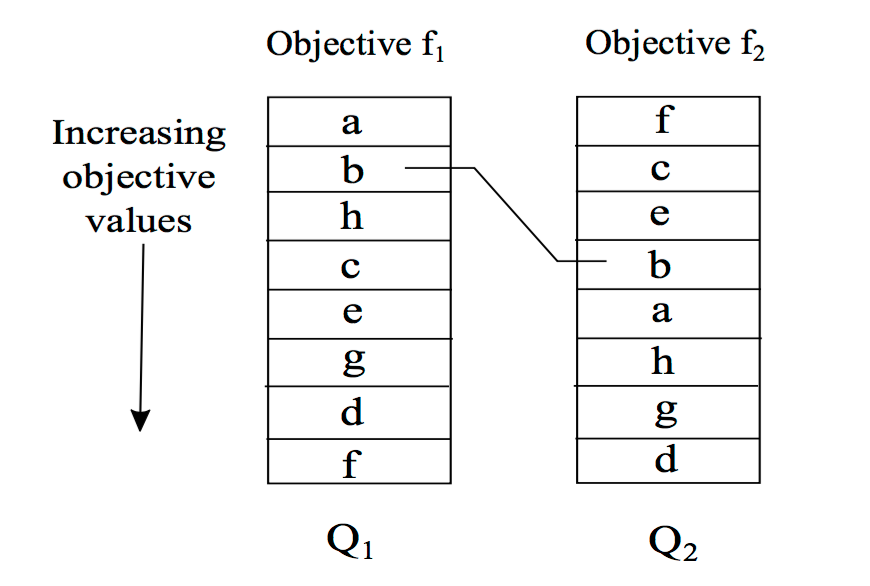
\includegraphics[width=8cm]{pic/bos_pic}
\caption{На рисунке представлены отсортированные списки по критерию f1 и f2. Точка b будет сравниваться только с точкой a и в последствии ее ранг не будет меняться.}
\label{bos_descr}
\end{center}
\end{figure}

Более детальное описание алгоритма не так существенно, так как алгоритм BOS встраивается в алгоритм Fast, и его внутреннее устройство не очень интересно. 



\section{Недостатки существующих алгоритмов}

Все описанные выше алгоритмы имеют разные асимптотики времени работы. 

Квадратичные алгоритмы и алгоритмы с большей асимптотикой работают медленно на больших данных, однако при небольшом
размере входного множества способны завершать работу быстрее алгоритмов ``разделяй и властвуй'' из-за того, что те
вынуждены делать много дополнительной работы, которая оказывается лишней на таких небольших размерах входных данных.

Алгоритмы ``разделяй и властвуй'' имеют хорошую асимптотику. В случае алгоритма Буздалова, даже на самых плохих входных 
данных. Однако они начинают работать гораздо хуже, когда размерность задачи $M$ перестает быть константой, потому что 
экспоненциально зависят от его значения. Стоит признать, что случай больших $M$ довольно редко встречается на практике,
однако не явялется невозможным.

Последний из рассмотренных алгоритмов, алгоритм Роя, имеет интересную идею и показал хорошие результаты 
на практике. Однако теоретическое время его работы исследованно крайне плохо. Поэтому нельзя заране утверждать, всегда 
ли он лучше существующих алгоритмов.


\section{Постановка задачи}

Задача данной работы состоит в разработке нового гибридного алгоритма недоминирующей сортировки и разивается на подзадачи: 
\begin{itemize}
	\item Выбрать наиболее подходящие для гибридизации алгоритмы.
	\item Основываясь на практических экспериментах на разных видах входных данных, оценить время обработки каждым
	выбранным алгоритмом.
	\item Выдвинуть предположение о том, как и в какой момент менять стратегию сортировки. 
	\item Проверить предположение
	\item Сформулировать и реализовать гибридный алгоритм.
\end{itemize}
